\documentclass[UTF8]{ctexart}
\usepackage[UTF8]{ctex}
\usepackage{hyperref}
\usepackage{graphicx}

\begin{document}


\begin{center}
    Lizenziert unter CC BY-SA 4.0. Für Urheber, Quellen und Lizenzinformationen, siehe:\\
    \href{https://github.com/thomasgassmann/eth-cheatsheets}{github.com/thomasgassmann/eth-cheatsheets}

    GITCOMMIT
\end{center}


% TODO: clean up, use anki for some of these things

\section{Ausprache}

\subsection{Ausnahmen}

\begin{itemize}
    \item Folgt nach dem Wort 不 bù eine Silbe in einem vierten Ton, dann wird bù nicht bù,
    sondern bú im zweiten Ton ausgesprochen. Und den Tonwechsel muss man
    schreiben. Z.B. bú shì
    \item wenn zwei Silben im dritten Ton nebeneinander stehen die erste Silbe im zweiten
    Ton gelesen ABER NICHT geschrieben wird
    \item 还是 kann auch hái shi gelesen werden.
\end{itemize}

\subsection{不}

Obige Ausnahme gilt für 不. Ausserdem kann 不 auch im neutralen Ton gelesen werden (bspw. bei 对不起).

\subsection{一}

一 is pronounced in the first tone when it stands alone. It is pronounced in the fourth tone when it precedes a first, second, or third tone. However, it is pronounced in the second tone when it precedes a fourth tone.

When 一 (yī) appears as an ordinal number (as in "first"), or as a number in a series, address, or date, it is pronounced without the tone change (regular first tone "yī")

\begin{itemize}
    \item 一 (yī)
    \item 一百 (yìbǎi)
    \item 一万 (yíwàn)
\end{itemize}

Wenn auf 一 ein ZEW folgt, wird es im vierten Ton ausgesprochen.

Wenn man eine Telefonnummer sagt, darf man nicht yī sagen, sondern muss yāo sagen (und schreiben 幺).

\subsection{两}

两 wird generell verwendet als eine Zähleinheit. 二百 wird nur verwendet falls exakt 200 gesagt werden soll. 两百 ist auch möglich und wird generell bevorzugt. 二百零一 ist nicht möglich, nur 两百零一 ist möglich.

\subsection{Schwacher Ton}

Siehe S.77 in Zhongguohua für richtige Aussprache und Höhe.

\section{Grammatik}

\subsection{的 und 得}

的 kann bei einsilbigen Attributen weggelassen werden (z.B. Farben).

得 ist ein Modalkomplement, beschreibt ein Verb. Immer Verb + 得 + Komplement. Da 得 immer nach einem Verb kommen muss, muss man das Verb für das Objekt wiederholen. Bspw. 他(说)汉语说得很快。

Es gibt einen Unterschied zwischen 他说很快的汉语 (schnelles Chinesisch) und 他说汉语说得很快 (spricht schnell Chinesisch).

Das erste Verb kann normalerweise weggelassen werden (他汉语说得很好).

\subsection{Satzstruktur}

Immer Vorfeld, Subjekt, Angabe, Prädikate, Objekt, Modalpartikel.
吗 ist beispielsweise ein Modalpartikel. 怎么 kommt immer vor dem Verb. Ein Objekt kann auch ein Objektsatz sein, welcher wiederrum nach derselben Struktur aufgebaut ist.

Immer "grosse" Zeitangabe zuerst ins Vorfeld.

Beispiele:

\begin{itemize}
    \item 有时候我一个月挣400块钱
    \item 从星期一到星期五图书馆从十点到十二点开门
\end{itemize}

In der Angabe steht Zeitangabe immer vor Ortsangabe.

\subsection{Thema Rhema}

Der Satz 她用/花 300 块付房租 ist ein sogenannter Satz mit «Verben in Serie». Hierbei besteht der Satz aus einem Subjekt mit einer Aneinanderreihung von Verben (und Objekten). Im Deutschen werden solche Sätze oft mit «um zu» Sätze oder finalen Sätzen übersetzt. Den selben Satz kann man aber auch folgendermassen sagen: 付房租她用/花 300 块钱。Dies nennt man «Thema Rhema». Die bekanntere Information
(Thema) wird an den Satzanfang gestellt. Auf Deutsch wäre dies etwa: «Was die Wohnungsmiete anbelangt: Sie gibt 300 Franken aus.»

\subsection{给/向/根}

给 kann verwendet werden um ein Objekt in die Angabe zu schieben. Beispielsweise gibt es in 你给我发短信吧 zwei Objekte, deshalb können wir ein Objekt (我) mit 给 in die Angabe stellen. Die Angabe ist dann 给我. Siehe auch Video auf OLAT (2022-10-17).

Dasselbe geht auch mit 向, bspw. 她向我道歉.

\begin{itemize}
    \item 他晚上给孩子洗澡
    \item 他向我道歉
    \item 他明天想和我见面 / /他想明天和我见面
    \item 我想和她结婚
\end{itemize}

\subsection{Verben mit zwei Objekten}

Die Verben 给,问 und 教 können zwei Objekte haben.

Beispiel: 老师教学生汉字。\\
他问老师问题。

\subsection{Prozente}

人口百分之八十是中国人。 80 Prozent der Bevölkerung sind Chinesen.\\
Mit Komma: 百分之二十二点五。 22,5 Prozent.

\subsection{Adjektivprädikate}

Siehe auch Video. Adjektive brauchen 很,太。。。了,非常. Ansonsten ist bspw. 你的中文好 komparativ. 你的中文很好 ist dann nicht komparativ. Um herauszufinden ob wirklich 很 gemeint ist auf Aussprache achten (wenn wirklich "sehr" gemeint ist, wird 很 stärker betont).

\subsection{Nominalprädikate}

Bspw. 他16岁. 岁 hat eine prädikative Funktion.

Bei der Verneinung braucht man ein 是. 他不是16岁. 他不16岁 ist falsch.

Auch beim Geld (bspw. 一条蓝裤子一百二十块钱, kein 是)

\begin{itemize}
    \item 几点
    \item 块钱
    \item 岁
    \item 多大
    \item 多少钱
\end{itemize}

\subsection{Zweiteilige Verben}

Zweiteilige Verben sind lexikalisch zweigeteilte Verben, die aus einem verbalen und einem nominalen Teil bestehen, semantisch aber eine Einheit bilden. Orthografisch wird zusammengeschrieben, wenn der verbale Teil und der nominale Teil
einsilbig ist.

\begin{itemize}
    \item 做饭
    \item 看书
    \item 洗澡
\end{itemize}

Zwischen verbalem und nominalem Teil kann man auch Dinge (keine Objekte, aber Zeitdauer (kein Zeitpunkt oder Zeitangabe) bspw. erlaubt) einfügen:

\begin{itemize}
    \item 洗两次澡
    \item 见一次面
\end{itemize}

Bei zweiteiligen Verben ist das Objekt im Satz schon belegt weshalb man die Angabe verwenden muss.

\begin{itemize}
    \item FALSCH: 我打电话她, RICHTIG: 我给她打电话
    \item FALSCH: 王先⽣结婚她, RICHTIG: 王先⽣和她结婚
    \item FALSCH: 妈妈洗澡孩⼦, RICHTIG: 妈妈给孩⼦洗澡
\end{itemize}

Das Modalverb kommt zuerst, bspw. 我想和她结婚, nicht 我和她想结婚.

\subsection{了}

Sätze mit 了 werden mit 没有 verneint.

\subsection{Lokativ}

Für die Angabe wird ein Ort vorrausgesetzt. Ist es kein Ort, kann man es zu einem Lokativ machen mit 那儿,这儿,家.

Bspw. 在个体户买衣服砍价 ist falsch, muss 在个体户那儿买衣服砍价 sein, denn 个体户 ist kein Ort.\\

\subsection{Mal kurz...}

Verb zweimal wiederholen für Bedeutung "mal kurz"

看看: mal kurz schauen

\subsection{很}

多 und 少 immer mit 很.

\subsection{有点儿}

有点儿: vor Adjketiven und Verben, man kann auch 有一点儿 sagen.

一点儿: vor Nomen

一点儿 kann auch \textbf{nach} Adjketiven stehen, dann wird es komparativ. (bspw. 长一点儿). 


\subsection{ZEW}

ZEW verwenden bei:

\begin{itemize}
    \item Zahlwort 三,十,五十
    \item Demonstrativpronomen 这, 那
    \item Fragewort (welche/r/s), 哪
    \item Fragewort (wie viel) 几 (BEI 多少 DARF KEIN ZEW VERWENDET WERDEN)
\end{itemize}

Liste:

\begin{itemize}
    \item 个: allgemein (bspw. 哪个学生)
    \item 本: Bücher, alle Dinge die wie Bücher gebunden sind (几本书)
    \item 种: Sprachen (三种语言)
    \item 张: flache (dünne) Gegenstände (四张照片)
    \item 位: höflich für Personen (一位老师)
    \item 家: Firmen (三家公司)
    \item 件: Kleidung / Oberteil (毛衣,衬衫,上衣,T-恤)
    \item 位: Personen, respektvoller (三位老师)
    \item 口:Personen im gleichen Haushalt
    \item 双:Paare (Schuhe, Socken)
    \item 条:Dinge die lang sind (Schlange, Hose, Rock), 围巾
    \item 顶:Hüte
    \item 套:Set (西服)
    \item 块:Stücke (Kuchen, 手表)
    \item 副:Brillen, Handschuhe
    \item 只:手镯
    \item 根: 皮带
    \item 所:学校
    \item 节:课 (lesson)
    \item 门:课 (course)
    \item 堂:课 (lesson)
\end{itemize}

ZEW mit zwei ist immer 两+ZEW. Nie 二.

\subsection{Kleidung}

Anziehen: 穿,戴,系.

\begin{itemize}
    \item 穿:Generell.
    \item 戴:Accessories (Hüte, Brillen, etc.)
    \item 系:tragen (umbinden)
\end{itemize}

\subsection{认识}

认识 wird mit Personen verwendet, 知道 mit Dingen. Es gibt aber Ausnahmen:

\begin{itemize}
    \item 我认识XY汉字.
\end{itemize}

\subsection{Alter}

Für Kinder: 几岁

Jugendliche und Erwachsene: 多大

ältere Menschen: 多大岁数

\section{Geographie}

Seite 70-72 im Buch Provinzen mit Hauptstädten und Aussprache. Karte auf Seite 48.


\subsection{Richtungen}

Dasselbe für Norden, Süden, etc.:

\begin{itemize}
    \item Im Norden von: 北方
    \item nördlich von: 北边
\end{itemize}

Für Nordosten, Südosten, etc. schreibt man zuerst W/E und erst dann N/S. 方 kann weggelassen werden wenn schon 2 Silben vorhanden sind (bspw. 西藏在中国西南).

\section{Zeit}

点 in 现在几点 ist auch ein Zähleinheitswort.

\subsection{Wochentage}

Man verwendet 星期{一,二,三,四,五,六,天/日} oder 周{一,二,三,四,五,六,日}.

\subsection{Progressiver Aspekt}

Ähnlich wie "-ing" Form in Englisch. Es gibt drei Möglichkeiten:

\begin{itemize}
    \item ...呢:\\他吃饭呢
    \item 在...呢:\\他在吃饭呢
    \item 正(在)...(呢):\\他正(在)吃饭(呢)
\end{itemize}

Verwendet wird dazu auch oft 的时候 (während):

安娜睡觉的时候,老马在起床(呢)

\section{Geld}

Bei zwei Einheiten ist die zweite Einheit optional. Bspw. 一块五(毛)

Wenn es nur eine Einheit ist, muss man noch 钱 hinzufügen. Bspw. 五百块钱

\section{Zahlen}

Nullen hintendran darf man weglassen. Ansonsten immer mit 零 "auffüllen". Bei Zehnern darf man Zahl am Ende weglassen.

\begin{itemize}
    \item 101: 一百零一
    \item 120: 一百二(十)
\end{itemize}

Siehe auch Video auf OLAT (2022-10-17).

Man kann auch 一万万 anstelle von 一亿 verwenden.

Um "mehr als" auszudrücken, verwendet man 多 direkt nach der Zahl, bspw. 我花一千多块钱。

Um "ungefähr" auszudrücken kann man 左右 oder 差不多 verwenden. 左右 kommt hinter der Zahl, 差不多 vor der Zahl.

\section{Farben}

Basisfarben können ohne 色 geschrieben werden, andere Farben immer mit 色. Bspw. 米色 aber nicht 米. Auch bei zweisilbigen Farben braucht es kein 的.

\section{Schriftzeichen}

Man teilt einzelne Zeichen in Phonetikum und Signifikum/Radikal auf.

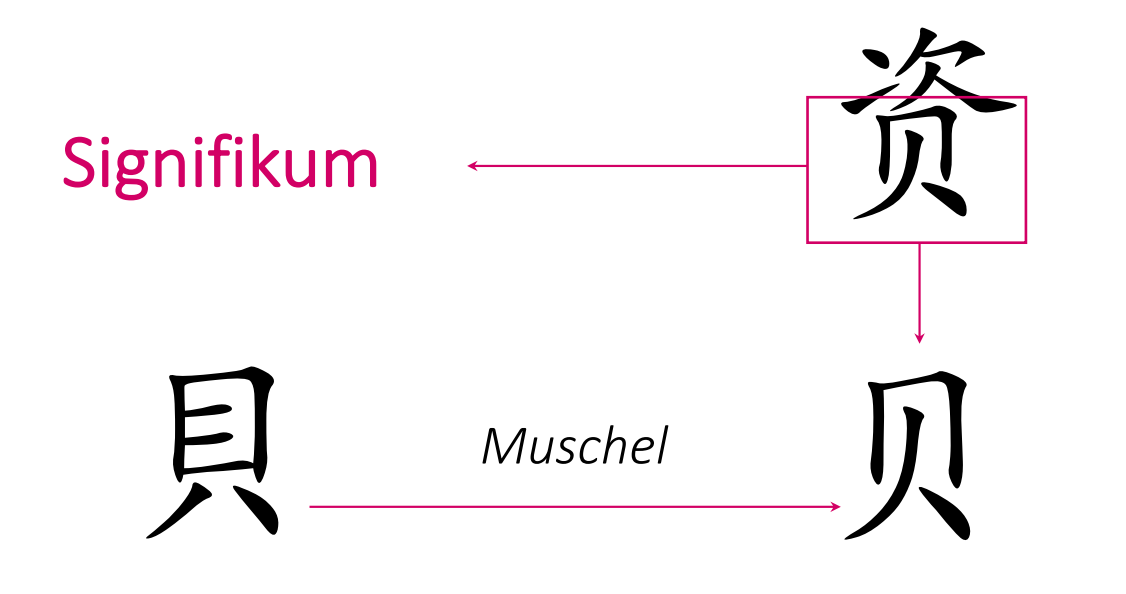
\includegraphics[width=\linewidth]{signifikum.png}

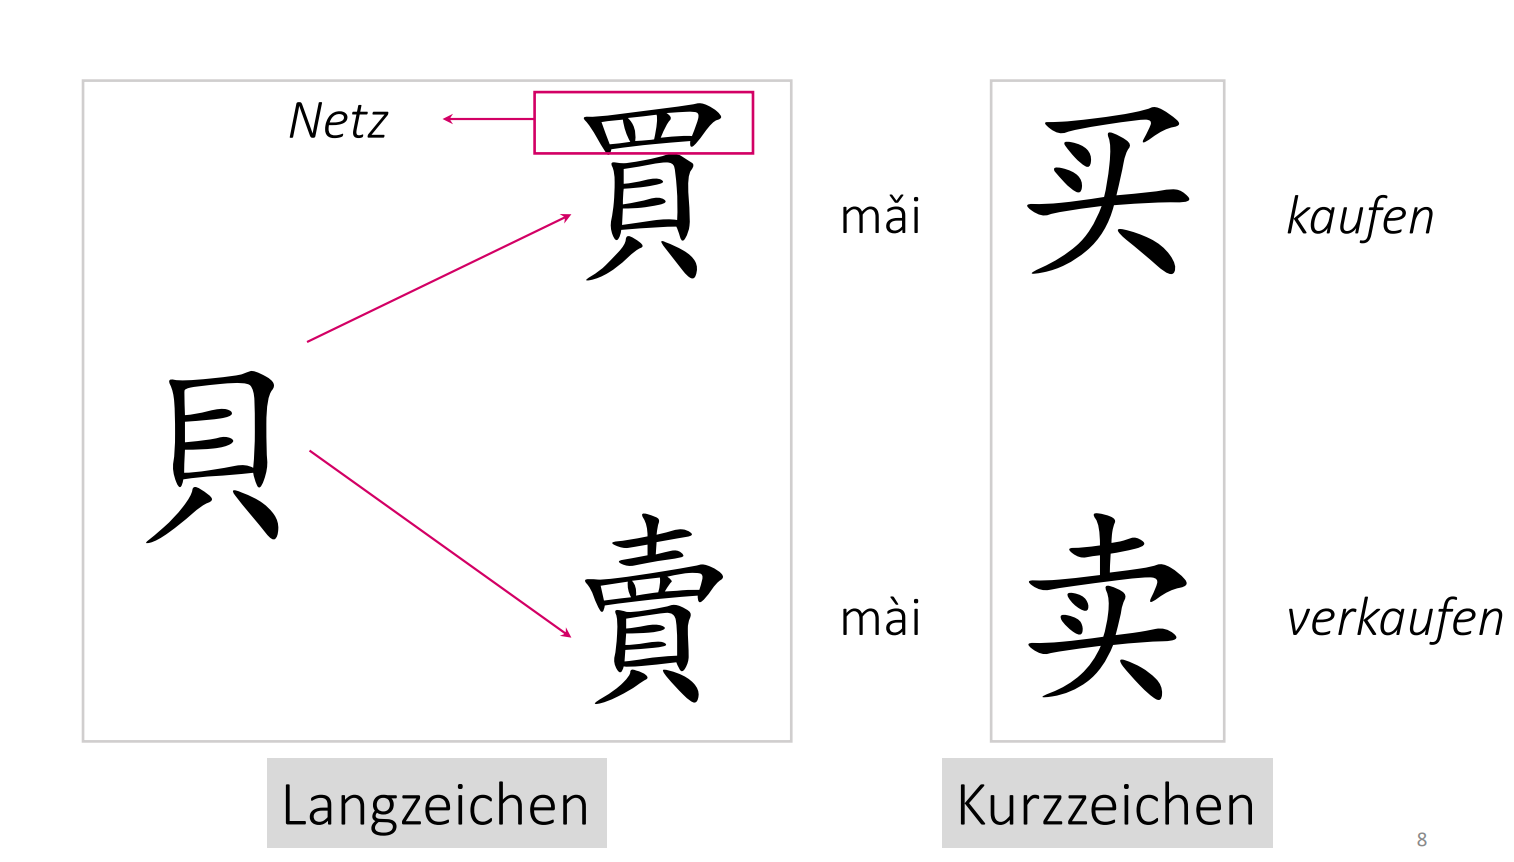
\includegraphics[width=\linewidth]{mai.png}

\end{document}
